% !TEX root = ../MasterThesis_Onoe.tex
% 上記はただのコメントではなく親ファイルの場所を教えているので
% 消してしまうとファイルごとのタイプセットができなくなるので注意。
% 親ファイル名を変更したときはここも変更する。

\chapter{序論} \label{sec:Intruduction}
 本章では、はじめに1.1節で素粒子とそれらに働く相互作用を説明する標準模型(The Standard Model, SM)について述べる。そして1.2節にて将来の電子陽電子ヒッグスファクトリーである、国際リニアコライダー計画(International Linear Collider, ILC)の概要に触れたのち、1.3節でILCが探索する物理、1.4節でILCのについて述べる。
\section{素粒子標準理論}
 素粒子とは、物質を構成している究極要素をさす名称である。そして素粒子物理学は、それら構成要素とその間に働く相互作用の性質を解明する学問である。現代の素粒子物理学では、すべての現象を説明するための基本的な枠組みとして図\ref{sm}のような標準模型を掲げており、これは現時点の実験データと高い精度で一致することが確認されている。\\

\begin{figure}[htbp]
	\begin{center}
 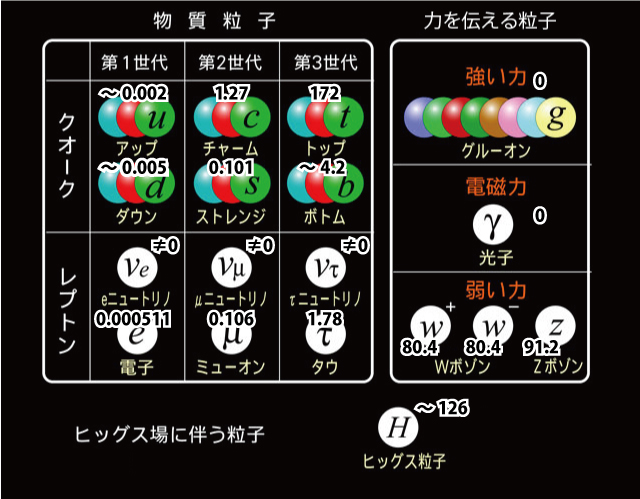
\includegraphics[keepaspectratio, scale=0.4]
 	{Figure/Introduction/sm.jpg}
 		\caption{素粒子の標準模型}
 		\label{sm}
	\end{center}
\end{figure}

 標準理論は、主に次に挙げる2つの公理に沿って記述されている。1つ目に、物質の究極要素である素粒子はクォークとレプトンというスピン1/2のフェルミオンである。2つ目に、素粒子の相互作用はゲージ粒子によって記述され、標準理論における相互作用は電磁相互作用・弱い相互作用・強い相互作用の3つである。\\
 物質の化学的性質を失わない最小単位は分子であり、分子はさらに原子の組み合わせによって構成されている。そして原子は原子核と電子によって構成されており、原子核は陽子と中性子のような核子からなっている。この核子を構成するものがクォークであり、標準模型においては6種類存在する。また同様に素粒子であり、核力のような強い相互作用をしないものをレプトンと呼び、同様に6種類存在する。クォーク・レプトンともに3つの世代と2つの電荷タイプをもっており、世代の高い粒子ほど重いため弱い相互作用により低い世代のクォークへと崩壊する。\\
 素粒子の相互作用を媒介するスピン1のゲージ粒子には、フォトン・Wボソン、Zボソン、グルーオンの4種類がある。このうち電磁相互作用と弱い相互作用は統一され電弱相互作用と呼ばれており、

標準模型は物質を構成する粒子であるフェルミオンと力を媒介する粒子であるボソンから構成される。またフェルミオンは、陽子や中性子を構成する6種類のクォークと電子やニュートリノなどのレプトンに大きく分けられる。クォーク、レプトンはそれぞれ電荷によって2つに分けられ、さらに世代によって3つに分けられる。

\section{国際リニアコライダー計画: ILC}

\section{ILCの物理}

\subsection{新物理探索}

\section{ILCにおける検出器}

\subsection{Particle Flow Algorithm: PFA}

\subsection{International Large Detector: ILD}

\subsubsection{飛跡検出器}

\subsubsection{電磁カロリメータ}

\subsubsection{ハドロンカロリメータ}

\subsubsection{ミューオン検出器}

\section{ILCにおける物理解析}

\subsection{事象再構成}

\section{本研究の目的}